
\section{Training Datasets}\label{subsec::datasets}

In Figure~\ref{fig::example_mnist_settings}, Figure~\ref{fig::example_celeba}, Figure~\ref{fig::example_rgbd}, and Figure~\ref{fig::example_nyu}, we show several example images of the training images used for the pair image generation tasks in the experiment section. Table~\ref{tbl::dataset_digit_count}, Table~\ref{tbl::dataset_attr_count}, Table~\ref{tbl::dataset_rgbd_count}, and Table~\ref{tbl::dataset_nyu_count} contain the statistics of the training datasets for the experiments.

\begin{figure}[tbh!]
\centering
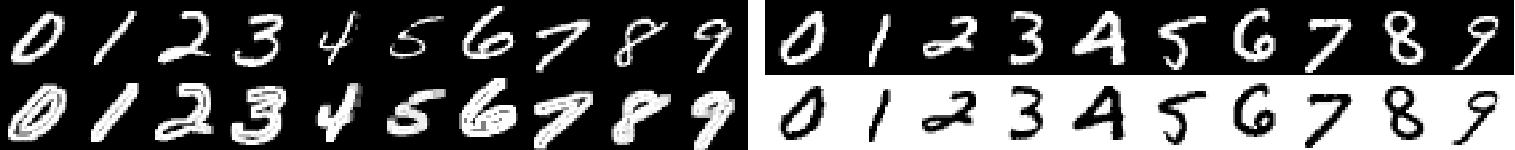
\includegraphics[trim=0.00in 0.0in 0.00in 0in,width=1.0\textwidth]{example_mnist_settings.pdf}
\caption{Training images for the digit experiments. Left (Task $\mathbb{A}$): The images in the first row are from the original MNIST digit domain, while those in the second row are from the edge image domain. Right (Task $\mathbb{B}$): The images in the first row are from the original MNIST digit domain, while those in the second row are from the negative image domain.}
\label{fig::example_mnist_settings}
\vspace{1mm}
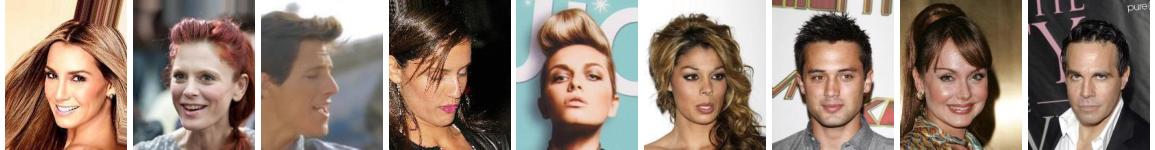
\includegraphics[trim=0.00in 0.0in 0.00in 0in,width=1.0\textwidth]{example_celeba.pdf}
\caption{Training images from the Celeba dataset~\cite{liu2015deep}.}
\label{fig::example_celeba}
\vspace{1mm}
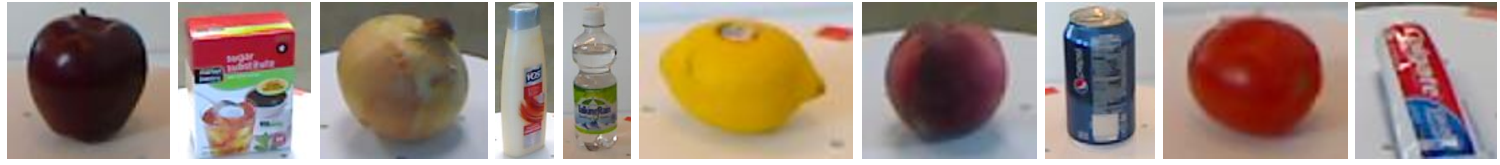
\includegraphics[trim=0.00in 0.0in 0.00in 0in,width=1.0\textwidth]{example_rgbd.pdf}
\caption{Training images from the RGBD dataset~\cite{lai2011large}.}
\label{fig::example_rgbd}
\vspace{1mm}
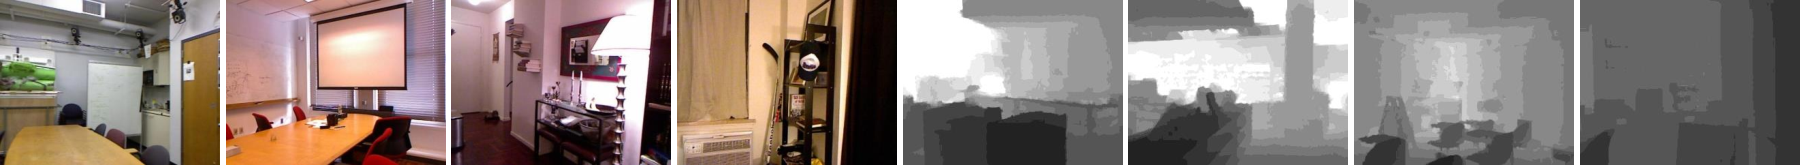
\includegraphics[trim=0.00in 0.0in 0.00in 0in,width=1.0\textwidth]{example_nyu.pdf}
\caption{Training images from the NYU dataset~\cite{silberman2012indoor}.}
\label{fig::example_nyu}
\end{figure}
\begin{table}[tbh!]
\centering
{ 
\caption{Numbers of training images in Domain 1 and Domain 2 in the MNIST experiments.}
\label{tbl::dataset_digit_count}
\begin{tabular}{ccc}
\hline
 & Task $\mathbb{A}$ 						 & Task $\mathbb{B}$ \\
 & Pair generation of digits and & Pair generation of digits and \\
 & corresponding edge images     & corresponding negative images\\ 
\hline
\# of images in Domain 1 & 30,000 & 30,000 \\
\# of images in Domain 2 & 30,000 & 30,000 \\
\hline
\end{tabular}}
\centering
{ 
\vspace{4mm}
\caption{Numbers of training images of different attributes in the pair face generation experiments.}
\label{tbl::dataset_attr_count}
\begin{tabular}{crrr}
\hline
Attribute & Smiling & Blond hair & Glasses\\
\hline
\# of images with the attribute & 97,669 & 29,983 & 13,193\\
\# of images without the attribute & 104,930  & 172,616 & 189,406\\
\hline
\end{tabular}}
\centering
{ 
\vspace{4mm}
\caption{Numbers of RGB and depth training images in the RGBD experiments.}
\label{tbl::dataset_rgbd_count}
\begin{tabular}{cc}
% \hline & RGBD objects \\
\hline
\# of RGB images   & 93,564 \\
\# of depth images & 93,564 \\
\hline
\end{tabular}}
\centering
{ 
\vspace{4mm}
\caption{Numbers of RGB and depth training images in the NYU experiments.}
\label{tbl::dataset_nyu_count}
\begin{tabular}{cr}
% \hline & NYU indoor scene\\
\hline
\# of RGB images   & 514,192 \\
\# of depth images & 1,449 \\
\hline
\end{tabular}}
\end{table}
